\documentclass[tt1]{penoverslag}

%%% PACKAGES
\usepackage{lipsum}
\usepackage{gensymb}
\usepackage [dutch] {babel}
\usepackage{graphicx}
\usepackage{amsmath}
\usepackage{listings}
\usepackage{subcaption}


\begin{document}

\team{Zilver} % teamkleur
\members{Sam Gielis\\
         Sophie Marien\\
         Toon Nolten\\
         Nele Rober\\
         Gerlinde Van Roey\\
         Maxim Van Mechelen} % teamleden

\maketitlepage

\begin{abstract}
Het P\&O-project heeft als doel vier autonome robots \textit{Team Treasure Trek} te laten spelen. De robots moeten hierbij in een onbekende doolhof op zoek naar een bepaald voorwerp. Voor elke robot wordt een ander voorwerp gereserveerd. Wanneer een robot zijn voorwerp gevonden heeft, komt hij te weten met welke robot hij moet samenwerken. Elk duo moet de twee voorwerpen bij elkaar brengen. Wie hier eerst in slaagt, wint. Dit verslag beschrijft de invulling die team Zilver aan het project gaf.\\

De robot is voorzien van een lichtsensor, een infraroodsensor en een ultrasone sensor. De laatste twee staan vast gemonteerd en kunnen niet onafhankelijk van de robot bewegen. De lichtsensor kan wegklappen opdat de robot over de wip kan rijden. Verder is de robot voorzien van een strook klittenband waarmee hij het voorwerp, ook voorzien van klittenband, kan oprapen. Dit gebeurt door het voorwerp te klemmen tussen de muur en de robot zodat de klittenband goed vast zit.\\

De robot kan een doolhof verkennen en er een map van bijhouden. Wanneer een tegel gevonden wordt die mogelijk een voorwerp bevat, zal deze eerst nagekeken worden alvorens verder het doolhof te verkennen.\\

Via RabbitMQ kunnen de robots en simulators met elkaar communiceren.\\

Een computerprogramma simuleert de werking van robots. Deze simulator kan vier robots tegelijk simuleren of kan in hybride vorm gebruikt worden (waarbij \'e\'en fysieke en drie virtuele robots gebruikt worden). De gesimuleerde robots gedragen zich volledig analoog aan de fysieke robot.
\end{abstract}

%figuur robot
\begin{figure}[!hb]
\begin{flushright}
    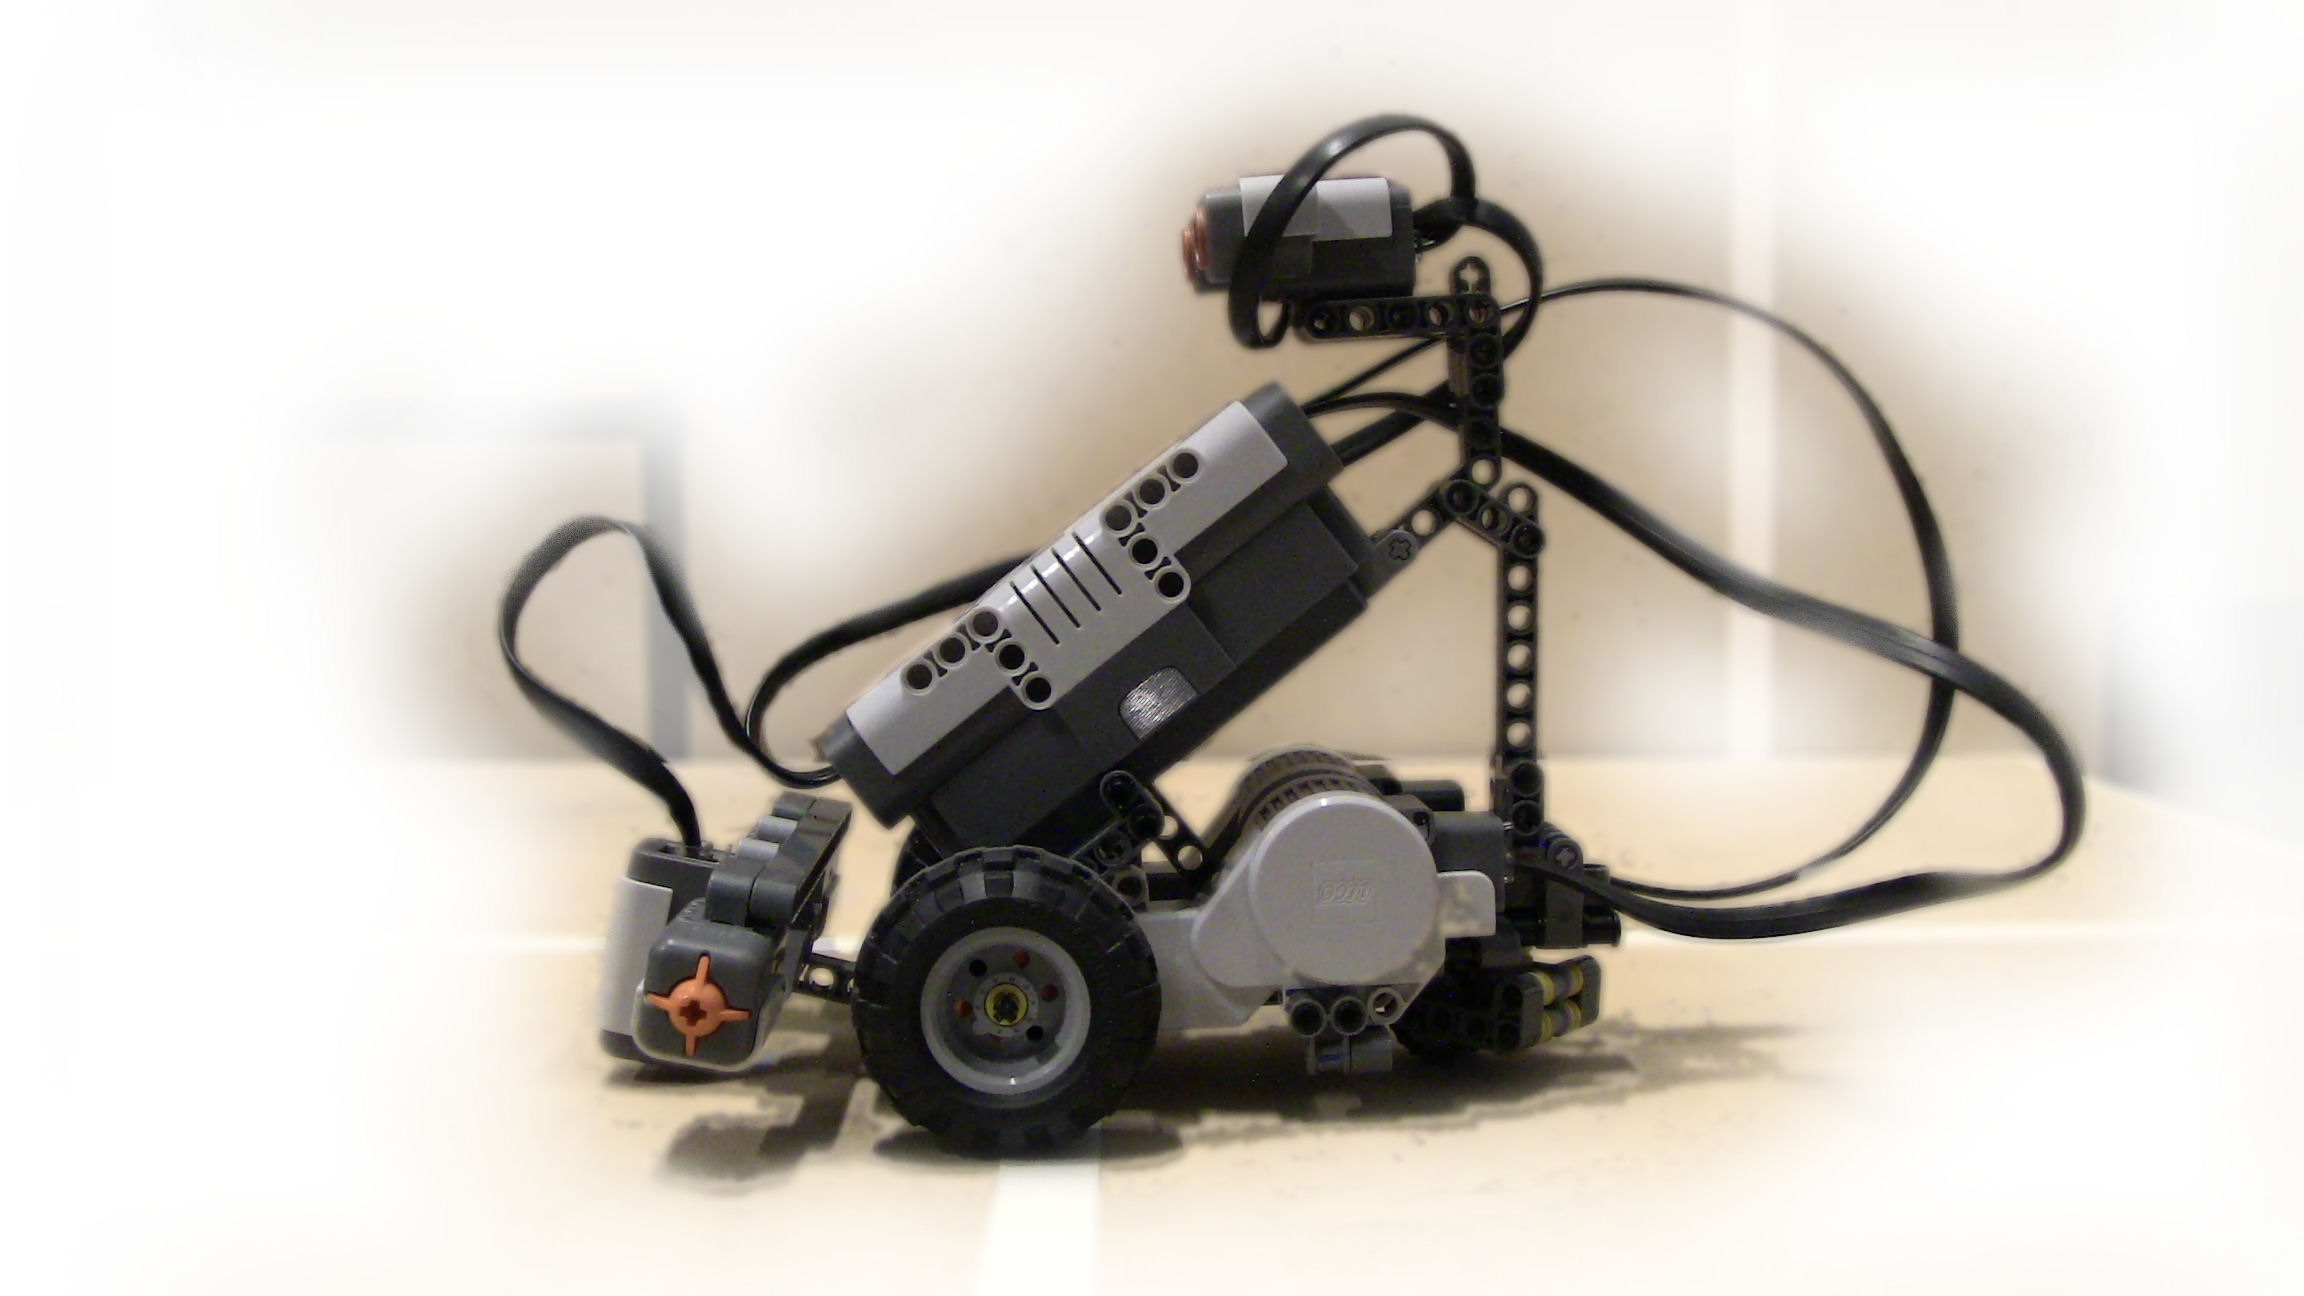
\includegraphics[width=0.8\textwidth]{robotFP2}
    \label{fig:robotFP2}
\end{flushright}
\end{figure}

\newpage
\setcounter{tocdepth}{2}
\tableofcontents

\newpage


% == INLEIDING == %
\section{Inleiding} % 4 ok
\label{ssec:inl}
In het kader van het vak `Probleemoplossen en Ontwerpen: computerwetenschappen' wordt gewerkt rond autonome intelligente robots. Verschillende teams bouwen en programmeren een robot met behulp van LEGO Mindstorms \cite{mindstorms}. Deze robot moet uiteindelijk samen met drie andere robots volledig autonoom \textit{Team Treasure Trek} kunnen spelen.\\

De eerste demonstratie bestaat erin de robot te laten rondrijden in een doolhof. De robot is in staat zijn voorwerp te zoeken en op te pikken terwijl de drie overige robots gesimuleerd worden. Bij het oppikken moet de robot dit laten weten aan zijn teamgenoot. Het is ook mogelijk met vier virtuele robots te werken. De virtuele robots communiceren met elkaar via RabbitMQ.\\


\section{Bouw robot}
\label{ssec:bouwrob}
LEGO Mindstorms \cite{mindstorms} biedt een bouwpakket voor een robot aan. Een NXT-microcomputer laat toe de robot te programmeren. Met behulp van leJOS \cite{leJOS} kan dit in Java.


\subsection{Fysieke bouw}
\label{ssec:fysb}

De fysieke bouw van de robot is grotendeels gebaseerd op die van het eerste semester. Enkele aanpassingen waren echter nodig om de robot aan de passen aan zijn nieuwe opdracht. De robot moet in staat zijn een voorwerp, met name een wc-rolletje, op te nemen en er zullen extra sensoren ingesteld moeten worden voor bijkomende hindernissen zoals het kunnen detecteren van andere robots, het detecteren van de wip, vaststellen of het voorwerp daadwerkelijk is opgepakt,... .  
Qua sensoren, zijn er twee veranderingen gebeurt ten opzichte van het eerste semester. De druksensoren aan weerszijde van de lichtsensor zijn weggehaald. Deze waren van nut om te detecteren wanneer er tegen een muur werd opgebotst tijdens het wittelijnalgoritme. Deze zijn echter nooit geimplementeerd en bleken ook niet nodig te zijn dus zijn deze voor dit semester eraf gehaald. 

De tweede aanpassing is een infraroodsensor\footnote{ervan uitgaande dat er een infraroodbal onder de wip ligt, kan deze sensor handig zijn om de stand van de wip te detecteren. Het is echter niet zeker of er gebruik gaat gemaakt worden van deze bal.} bovenop de robot. Deze infraroodsensor dient voor het detecteren van een infrarood balletje. Dit balletje wordt onder de wip geplaatst. Als de wip naar beneden staat zal het balletje achter de wip verdwenen zijn en niet gedetecteerd worden. Hierdoor weet de robot dat de wip naar beneden staat en dat hij doorkan. Als het balletje wel gedetecteerd wordt, weet de robot dat de wip omhoog staat en dat hij er dus niet over kan. \\

Om het voorwerp op te nemen zijn verschillende opstellingen mogelijk. Er moet rekening gehouden worden met de hinder die de extra omvang van het voorwerp teweeg kan brengen bij het voortbewegen van de robot.
Ook is het nuttig het voorwerp niet over de grond te laten slepen. Dit zorg voor extra wrijving en vergroot de kans dat het voorwerp valt. Ten laatste moet de robot een wip kunnen passeren. 
 
Deze zaken in beschouwing nemend, werd er aanvankelijk voor gekozen om een schep achteraan de robot te monteren om zo het voorwerp op te nemen. Dit geeft als voordeel de wip zonder probleem te kunnen passeren. Het probleem hiermee is dat de robot dan een te grote lengte krijgt waardoor het onmogelijk werd voor de robot om te draaien op een tegel zonder tegen een muur aan te botsen. \\

Daarom werd de opstelling waarin de schep van de robot vooraan gemonteerd wordt, verkozen. De schep is opgebouwd uit een deel van een wc-rol. Dit heeft namelijk de ideale vorm om het voorwerp, het wc-rolletje, op te nemen. 
Het voorwerp wordt omringd met velcro. Dit biedt een extra ondersteuning om het voorwerp steviger vast te houden. 




% == ALGORITMES == %
\section{Algoritmes}
Voor volgende algoritmes wordt verwezen naar het verslag van het eerste semester. Deze algoritmes worden dit semester zonder aanpassingen opnieuw gebruikt.
\begin{itemize}
	\item Rechtzetten op een witte lijn
	\item Centreren aan de hand van twee muren
	\item Lezen van een barcode
	\item Vinden van het kortste pad
\end{itemize}

% == zoeken van het voorwerp == %
\subsection{Zoeken van het voorwerp} %
\label{ssec:algoZoek}
Om het voorwerp te vinden moet de robot aanvankelijk het doolhof verkennen. De robot gebruikt hiervoor een verken-algoritme. Elke tegel die de robot passeert, wordt gemarkeerd. Indien alle tegels gemarkeerd zijn, is de volledige doolhof doorzocht. Elke tegel houdt een boolean bij die deze markering voorstelt.

Bij elke tegel onthoudt de robot alle uitwegen (de naburige tegels). Vervolgens slaat hij de laatste nog niet bekeken uitweg in. Wanneer de robot op een doodlopend stuk komt, keert hij terug tot een kruispunt waar nog niet alle uitwegen van bekeken werden. De robot gebruikt het kortste-pad-algoritme om de weg naar dit kruispunt te bepalen.\\

Enkele optimalisaties werden doorgevoerd in het verken-algoritme. De genoemde aanpassing implementeert steeds ook de aanpassingen die eerder werden toegevoegd. Tabel~\ref{tab:resultVerken} geeft de resultaten van de aanpassingen weer. Figuur~\ref{fig:resultVerkenE} toont de gebruikte doolhoven en de uitvoering van het algoritme met aanpassing E. Er werd getracht het aantal draaiingen en afgelegde afstand te minimaliseren.

\begin{description}
\item[A] basisalgoritme zonder optimalisatie: draai bij elke tegel vier keer (eindig in startori\"entatie) en neem de laatste tile in de queue als volgende tile.
\item[B] neem steeds de buur die met het minst aantal rotaties bereikt kan worden als volgende tile.
\item[C] draai bij elke tegel slechts drie keer (eindig niet meer in startori"entatie).
\item[D] muren die vanuit een naburige tile reeds gedetecteerd werden, worden niet nog eens nagekeken.
\item[E] tiles waarvan de vier zijden al gekend zijn en geen `straight' zijn, worden niet meer bezocht (enkel `straights' kunnen barcodes bevatten, dus dit is geen probleem)
\end{description}

%resultaten lichtsensor
\begin{table}[!hb]
\begin{center}
    \begin{tabular}{ c ||  c | c | c | c }
     & \multicolumn{2}{|c|}{map 1}& \multicolumn{2}{|c}{map 2} \\
    optimalisatie & gedraaid & cm afgelegd & gedraaid & cm afgelegd\\ \hline \hline
    A & 14400 & 2160 & 10620 & 1080 \\ \hline
    B & 13770 & 1920 & 10800 & 1160 \\ \hline
    C & 11970 & 2000 & 9090 & 1080 \\ \hline
    D & 9180 & 2000 & 6570 & 1080\\ \hline
    E & 8820 & 1880 & 6570 & 1080\\
    \end{tabular}
    \caption{Verbeteringen aan het verkenalgoritme}
    \label{tab:resultVerken}
\end{center}
\end{table}

% figuren verkenning doolhof
\begin{figure}
\centering
	\begin{subfigure}[hb]{0.64\textwidth}
	\centering
		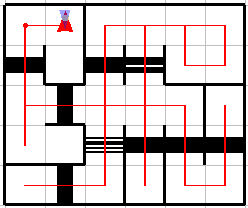
\includegraphics[width=\textwidth]{verkenMap1E}
		\caption{map 1}
	\end{subfigure}%
	\begin{subfigure}[hb]{0.36\textwidth}
		\centering
		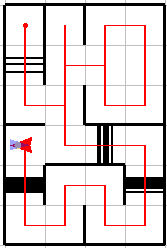
\includegraphics[width=\textwidth]{verkenMap2E}
	\caption{map 2}
\end{subfigure}
\caption[Verkennen van een doolhof]{Verkennen van een doolhof met implementatie van aanpassing E. Deze aanpassing maakt dat in map 1 niet alle tegels bezocht hoeven te worden. In map 2 doet deze situatie zich niet voor. Dit is te wijten aan de opbouw van de doolhof.}
\label{fig:resultVerkenE}
\end{figure}

Een extra optimalisatie geeft prioriteit aan het vinden van het voorwerp. Een voorwerp kan zich enkel bevinden op een `dead-end', voorafgegaan door een `straight' die een barcode bevat. Deze barcode identificeert het voorwerp. Wanneer een mogelijke voorwerp-locatie gevonden wordt, wordt zo snel mogelijk nagegaan of het om het juiste voorwerp gaat. In sommige gevallen is het niet mogelijk rechtstreeks naar de locatie te gaan omdat het doolhof daar nog niet verkend is. In dat geval wordt verder verkend in de richting van de locatie. De `dead-end' zelf hoeft niet bezocht te worden wanneer uit de barcode blijkt dat het niet om het juiste voorwerp gaat, zodat optimalisatie E nog steeds geldt.\\

Nadat het voorwerp gevonden is, probeert de robot zijn teamgenoot te contacteren. Indien de teamgenoot zijn voorwerp nog niet heeft of wanneer de mappen van beide robots nog niet combineerbaar zijn, gaat de robot verder met het verkennen van het doolhof. Hierbij wordt nog steeds prioriteit gegeven aan voorwerp-locaties. Deze bevatten immers unieke barcodes die het later makkelijker maken de mappen te combineren.

Als alternatief kan de robot zich naar het voorwerp van de teamgenoot begeven om daar op hem te wachten (niet te dicht bij om niet in de weg te staan). Deze extra optie wordt voorlopig nog niet ge\"implementeerd omdat nog niet duidelijk is in welke gevallen de strategie het best werkt.

% nog niet voor deze demo!
%\subsection*{Algoritme om zo snel mogelijk naar de andere robot te gaan}
%Hierbij dachten we aan het kortste-pad-algoritme. Dit zal wel nog aangepast moeten worden aan zowel draaien als vooruit rijden (draaien was nog niet in rekening gebracht).\\ Er moet ook nog rekening gehouden worden als de andere robot zou wegrijden. De robot mag hierdoor niet in een loop terechtkomen. Er zou moeten gecommuniceerd worden wie naar wie toerijdt, of dat er naar een gezamenlijke tegel moet gereden worden. \\
%Als de andere robot zou wegrijden zou er een afstand kunnen bijgehouden worden die dan opnieuw berekent wordt als de afstand niet kleiner wordt.

% == SOFTWARE == %
\section{Software}
\label{secc:softw}

\subsection{RabbitMQ}
\label{secc:RabbMQ}
Via RabbitMG wordt de communicatie met de andere robots verzorgt. RabbitMQ werkt via queue's. .. en nog verdere info

\subsection{GUI}


\subsection{Simulator}
\begin{itemize}
\item Beschrijving van de simulator.
\end{itemize}

\subsection{Software design}
\begin{itemize}
\item Geef hier een klassediagramma en een overzicht van de verschillende methodes.
\end{itemize}

\subsection{\ldots}
\ldots


% == BESLUIT == %
\section{Besluit}



\newpage
\makeappendix

\section{Demo 1}

\subsection{Resultaten}
\ldots

\subsection{Conclusies}
\ldots

\subsection{Oplijsting aanpassingen verslag}
Hier komt een summiere weergave van welke secties uit het vorige verslag gewijzigd werden.





\section{Beschrijving van het proces}
\begin{itemize}
\item Welke moeilijkheden heb je ondervonden tijdens de uitwerking?
\item Welke lessen heb je getrokken uit de manier waarop je het project hebt aangepakt?
\item Hoe verliep het werken in team? Op welke manier werd de teamco\"ordinatie en planning aangepakt?
\end{itemize}


\section{Beschrijving van de werkverdeling}
\begin{itemize}
\item Geef voor elk van de groepsleden aan aan welke delen ze hebben meegewerkt en welke andere taken ze op zich hebben genomen.
\item Rapporteer in tabelvorm hoeveel uur elk groepslid elke week aan het project gewerkt heeft, zowel tijdens als buiten de begeleide sessies. Geef ook totalen per groepslid voor het volledige semester.
\end{itemize}


\section{Kritisch analyse}
\begin{itemize}
\item Maak een analyse van de sterke en zwakke punten van het project. Welke punten zijn vatbaar voor verbetering. Wat zou je, met je huidige kennis, anders aangepakt hebben?
\end{itemize}



\newpage
\bibliographystyle{siam}
\bibliography{biblio.bib}

\begin{thebibliography}{9}
\bibitem{mindstorms}
\textit{Lego Mindstorms}:  Een uitbreiding op de LEGO bouwstenen waarmee kleine, aanpasbare en programmeerbare robots gebouwd kunnen worden. Een centrale besturingsmodule (`the brick') kan geprogrammeerd worden met verschillende programmeertalen. In eerdere versies werd een RCX gebruikt voor de brick, nu wordt met NXT gewerkt. De brick kan enkele motoren aandrijven. Bovendien kunnen er verschillende sensoren, o.a. een ultrasone sensor en een lichtsensor, aangesloten worden.  \mbox{[www.lego.com]} \mbox{[http://en.wikipedia.org/wiki/Lego\textendash Mindstorms]}

\bibitem{leJOS}
\textit{leJOS}: Een kleine Java Virtuele Machine die toelaat de NXT-brick te programmeren. leJOS voorziet verschillende klassen die o.a. de motoren aansturen en een bluetoothverbinding opzetten.  \mbox{[http://lejos.sourceforge.net/]}

\bibitem{A*}
\textit{A*}: Een optimaal zoekalgoritme. \textit{A*} kiest zijn volgende punt op basis van een kostenfunctie: de werkelijke kost om tot de beschouwde buur te geraken, plus de geschatte kost om van dat punt naar het doel te geraken. Met andere woorden, het algoritme combineert een heuristisch algoritme met een kostenalgoritme. Zie ook de cursus \textit{Artifici\"ele Intelligentie (H06U1A)} door Daniel De Schreye.

\bibitem{manhattan}
\textit{Manhattanafstand:} Deze heuristiek tekent vanuit het ene punt een horizontale lijn en vanuit het andere punt een verticale lijn. De gemeten afstand is die van het ene punt tot het snijpunt, plus die van het andere punt tot het snijpunt.\\
In de doolhof wordt geen rekening gehouden met muren.\\
De Manhattanafstand verwijst naar een gelijknamige stadsdeel in New~York~City~VSA). New~York werd in het jaar~1625 door de Nederlanders gesticht. De straten werden in dambordpatroon gelegd: `Avenues' van noord naar zuid en `Streets' van oost naar west.\\
\mbox{$[http://nl.wikipedia.org/wiki/Manhattan\_(New\_York)]$}\\ \mbox{$[http://nl.wikipedia.org/wiki/New\_York\_City]$}

\end{thebibliography}


\end{document}
